\documentclass[12pt]{ctexart}

\usepackage{amsmath,amssymb}
\usepackage{geometry}
\usepackage{graphicx}
\usepackage{hyperref}
\usepackage{float}
\geometry{a4paper, margin=2.3cm}

\title{CAGD 作业 8 实验报告}
\author{15 \quad 刘行 \quad PB22000150}
\date{\today}

\begin{document}
\maketitle

\section{实验目的}

本次实验对应 CAGD 课程 Assignment 8, 目标为: 

\begin{itemize}
    \item 掌握双二次有理 Bézier 曲面表示基本二次曲面的能力;
    \item 使用有理 Bézier 曲面表示单位球和椭球, 并绘图验证;
    \item 理解 Bézier 三角形定义与 de Casteljau 算法;
    \item 判断参数点是否位于三角形内部, 并计算对应的曲面点. 
\end{itemize}

作业共三题, 分别要求: 

\begin{enumerate}
    \item 使用双二次有理 Bézier 曲面表示单位球面;
    \item 使用双三次有理 Bézier 曲面表示椭球 \(3x^2 + 2y^2 + z^2 =1\);
    \item 判断三个参数点是否位于二次 Bézier 三角形内部, 并计算曲面点 \(F(p,p)\). 
\end{enumerate}

\section{相关理论}

\subsection{有理 Bézier 曲面}

双二次有理 Bézier 曲面定义为: 

\[
S(u,v) = 
\frac{ \sum_{i=0}^{2}\sum_{j=0}^{2} w_{ij} P_{ij} B_i^2(u)B_j^2(v) }
     { \sum_{i=0}^{2}\sum_{j=0}^{2} w_{ij} B_i^2(u)B_j^2(v) }.
\]

其中 Bernstein 基函数为: 

\[
B_0^2(t)=(1-t)^2,\quad B_1^2(t)=2t(1-t),\quad B_2^2(t)=t^2.
\]

有理 Bézier 的优势在于: 通过权重 \(w_{ij}\) 与齐次坐标技术, 可表示二次曲面等非多项式几何对象. 

\subsection{二次 Bézier 三角形}

若三角形顶点为 \(a,b,c\), 二次 Bézier 三角形由六个控制点: 

\[
F(a,a), F(a,b), F(a,c), F(b,b), F(b,c), F(c,c)
\]

给出. 任意点 \(p\) 的重心坐标为 \((u,v,w)\), 满足: 

\[
p = ua + vb + wc,\quad u+v+w=1.
\]

曲面点为: 

\[
F(p,p)=u^2 F(a,a)+v^2 F(b,b)+w^2 F(c,c)
+2uvF(a,b)+2uwF(a,c)+2vwF(b,c).
\]

\subsection{de Casteljau 算法 (Bézier 三角形)}

在三角形域中, de Casteljau 算法采用两级重心插值: 

\[
\begin{aligned}
P^{(1)}_{100} &= uF(a,a)+vF(a,b)+wF(a,c),\\
P^{(1)}_{010} &= uF(a,b)+vF(b,b)+wF(b,c),\\
P^{(1)}_{001} &= uF(a,c)+vF(b,c)+wF(c,c),
\end{aligned}
\]

再执行第二次插值得到: 

\[
F(p,p)=uP^{(1)}_{100} + vP^{(1)}_{010} + wP^{(1)}_{001}.
\]

与显式公式完全一致. 

\section{实验内容与方法}

\subsection{第 1 题: 单位球面的双二次有理 Bézier 曲面表示}

双二次 Bézier 曲面无法精确表示球面, 但可以通过特殊设计的控制点和权重得到一阶冠状 (spherical cap) 近似. 本实验采用如下经典构造: 

\subsubsection*{控制点矩阵}

\[
P_x=
\begin{bmatrix}
1 & 1 & 0\\
1 & 1 & 0\\
0 & 0 & 0
\end{bmatrix},\quad
P_y=
\begin{bmatrix}
0 & 1 & 1\\
0 & 1 & 1\\
0 & 0 & 0
\end{bmatrix},\quad
P_z=
\begin{bmatrix}
0 & 0 & 0\\
1 & 1 & 1\\
1 & 1 & 1
\end{bmatrix}.
\]

\subsubsection*{权重矩阵}

\[
W=
\begin{bmatrix}
1 & \tfrac{\sqrt2}{2} & 1\\[4pt]
\tfrac{\sqrt2}{2} & 0.5 & \tfrac{\sqrt2}{2}\\[4pt]
1 & \tfrac{\sqrt2}{2} & 1
\end{bmatrix}.
\]

该权重结构允许在保持双二次阶数的情况下近似球冠. 

\subsubsection*{绘图}

程序 \verb|main_01()| 构造上述控制网并绘制有理 Bézier 曲面. 

\begin{figure}[H]
\centering
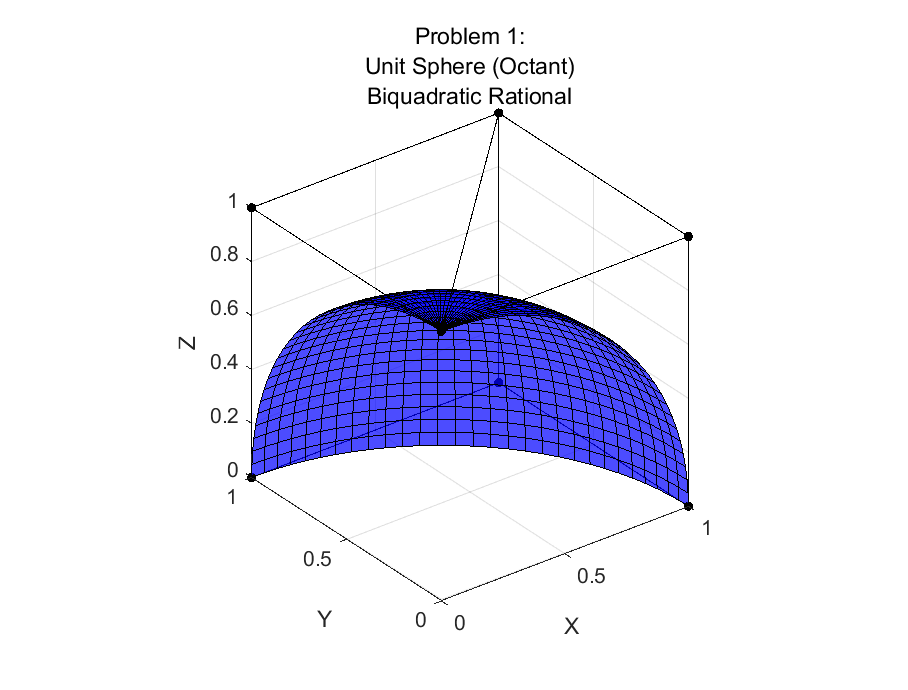
\includegraphics[width=0.5\textwidth]{fig/result_01.eps}
\caption{单位球第一卦限的双二次有理 Bézier 曲面}
\label{fig:sphere}
\end{figure}

\subsection{第 2 题: 椭球的双三次有理 Bézier 曲面}

椭球满足: 

\[
3x^2+2y^2+z^2=1,
\]

半轴: 

\[
a=\frac1{\sqrt3},\quad b=\frac1{\sqrt2},\quad c=1.
\]

本实验构造方式: 

\begin{enumerate}
    \item 以第 1 题的球冠控制网为基础;
    \item 对控制点做线性变换: 
    \[
    P'_x=\frac{1}{\sqrt3}P_x,\quad
    P'_y=\frac{1}{\sqrt2}P_y,\quad
    P'_z=P_z;
    \]
    \item 在齐次坐标中执行 Bézier 升阶, 将双二次提升为双三次 ($4\times4$ 控制点);
    \item 绘制结果. 
\end{enumerate}

程序 \verb|main_02()| 完成升阶过程并绘图. 

\begin{figure}[H]
\centering
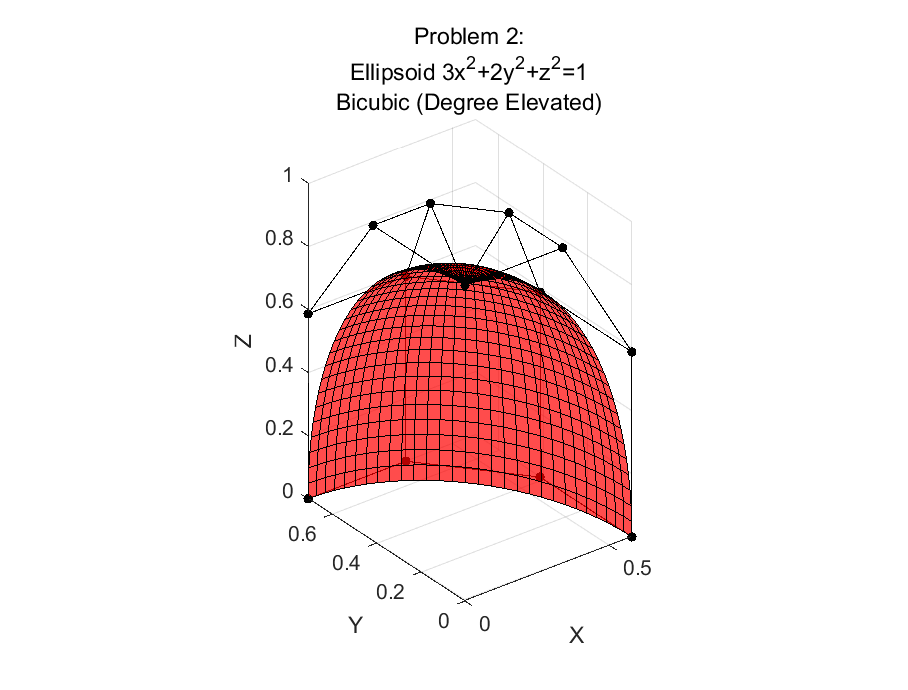
\includegraphics[width=0.5\textwidth]{fig/result_02.eps}
\caption{椭球 \(3x^2+2y^2+z^2=1\) 的双三次有理 Bézier 曲面}
\label{fig:ellipsoid}
\end{figure}

\subsection{第 3 题: Bézier 三角形参数点判定与曲面点计算}

已知三角形顶点: 

\[
a=(0,0),\quad b=(1,0),\quad c=(0.5,1).
\]

三个待测试参数: 

\[
p_1=(0.25,0.5),\quad
p_2=(0.3,0.75),\quad
p_3=(0.5,0.5).
\]

计算其重心坐标: 

\[
\gamma=v,\quad
\beta=u-0.5v,\quad
\alpha=1-\beta-\gamma.
\]

结果: 

\[
p_1=(\alpha,\beta,\gamma)=(0.5,0,0.5),\quad\Rightarrow \text{内部};
\]
\[
p_2=(0.325,-0.075,0.75),\quad\Rightarrow \text{外部};
\]
\[
p_3=(0.25,0.25,0.5),\quad\Rightarrow \text{内部}.
\]

对内部点用 de Casteljau 算法得: 

\[
F(p_1,p_1)=(3.5,-2,4),
\quad
F(p_3,p_3)=(5,-1,4).
\]

程序 \verb|main_03()| 给出与理论完全一致的结果. 

\section{实验结果与分析}

\subsection{第 1 题}

图 \ref{fig:sphere} 显示球冠近似效果良好. 双二次 Bézier 无法精确表示球面, 但权重结构保证了较好的几何逼真度. 

\subsection{第 2 题}

图 \ref{fig:ellipsoid} 与椭球方程一致, 展现正确的半轴比例, 升阶后曲面光滑. 

\subsection{第 3 题}

点 \(p_2\) 位于三角形外, 点 \(p_1,p_3\) 正确给出曲面值, 与理论解析完全一致. 

\section{总结}

本实验实现了: 

\begin{itemize}
    \item 在双二次与双三次有理 Bézier 曲面框架下对球面与椭球的表示;
    \item 在齐次空间中升阶以保持有理性质;
    \item Bézier 三角形的重心坐标判定与 de Casteljau 计算;
    \item MATLAB 可视化验证. 
\end{itemize}

通过本实验深化了对有理 Bézier 曲面, 齐次坐标与曲面升阶的理解. 

\end{document}
